A reach depth follows the flow through the reach, so like a lake stage it is a dependent variable that the Streamflow Routing (SFR) Package solves outside the groundwater flow matrix. The adjoint system is bordered in the same way as for a lake, described in Chapter~\ref{ch:lake}, with one equation per reach. What distinguishes the stream case is that those equations are not independent of one another: they carry the routing of water from reach to reach.

\section*{Reach equation}

\mf{} sets the depth $d$ of a reach so that the Manning discharge equals the mean of the flow entering and leaving it,

\begin{equation}
	\label{eqn:sfr-balance}
	q_{\mathrm{man}}(d) = \tfrac{1}{2}\left( Q_{\mathrm{in}} +
	Q_{\mathrm{out}} \right), \qquad
	Q_{\mathrm{out}} = Q_{\mathrm{in}} - Q_{\mathrm{leak}},
\end{equation}

\noindent where $Q_{\mathrm{leak}}$ is the exchange with the aquifer (L$^{3}$T$^{-1}$) and $d$ is the reach depth (L). For a reach without a cross section the wetted perimeter is the reach width, which carries no dependence on depth, so the discharge is a power of the depth,

\begin{equation}
	\label{eqn:sfr-manning}
	q_{\mathrm{man}}(d) = \frac{K w \sqrt{S}}{n}\, d^{5/3},
\end{equation}

\noindent with $w$ the width (L), $S$ the slope (dimensionless), $n$ Manning's roughness, and $K$ a unit conversion. The derivative needed for the border follows directly,

\begin{equation}
	\label{eqn:sfr-dqdd}
	\frac{\partial q_{\mathrm{man}}}{\partial d} = \frac{5}{3}
	\frac{q_{\mathrm{man}}}{d}.
\end{equation}

Equation~\ref{eqn:sfr-dqdd} is written in terms of the discharge \mf{} reports rather than rebuilding the rating from $K$, $w$, $S$, and $n$. The unit conversion in particular varies with the model's unit system, and taking the reported discharge makes the derivative correct without reproducing it.

Below a depth of $10^{-5}$ in model length units \mf{} smooths the discharge to zero. That smoothing is not reproduced, so a shallower reach is treated as carrying no flow.

\section*{Routing}

The flow entering a reach is the sum of the flows leaving the reaches upstream of it, apportioned by the diversion fractions specified for the network. The connectivity is that of the stream network itself, which identifies the reaches upstream of each reach.

Because $Q_{\mathrm{out}}$ of an upstream reach depends on that reach's depth and on its leakage, differentiating equation~\ref{eqn:sfr-balance} produces entries away from the diagonal in two places. The first couples one reach row to another,

\begin{equation}
	\label{eqn:sfr-updepth}
	\frac{\partial}{\partial d_{u}} \; \tfrac{1}{2} Q_{\mathrm{in}} =
	\tfrac{1}{2}\, \sigma \, \frac{\partial q_{\mathrm{man},u}}
	{\partial d_{u}},
\end{equation}

\noindent where $\sigma$ is the fraction of the upstream reach's outflow routed to this one (dimensionless). The second reaches back into the aquifer, because the flow leaving the upstream reach carries half of that reach's leakage,

\begin{equation}
	\label{eqn:sfr-uphead}
	\frac{\partial}{\partial h_{u}} \; \tfrac{1}{2} Q_{\mathrm{in}} =
	\tfrac{1}{2}\, \sigma \, \mathrm{HCOF}_{u}.
\end{equation}

The sign of equation~\ref{eqn:sfr-uphead} is easy to get wrong, and an error there is not obvious in the result: it produces sensitivities of a plausible magnitude that are wrong by a modest factor. Checking the assembled block against a finite-difference Jacobian is what identified it.

\section*{Flow-limited reaches}

A reach can be asked to lose more water than it carries. \mf{} limits the leakage to the available flow, and marks that state by leaving both the reach's \texttt{HCOF} and the change in its outflow at zero: the reach passes on nothing and its leakage no longer responds to the head beneath it.

The derivative structure changes accordingly. The reach's own depth no longer sets its leakage, so the coupling moves to the reaches upstream that supply it, and a correction appears that connects one aquifer cell directly to another, bypassing the reach equation. That correction is folded into the aquifer block of the bordered matrix rather than the border itself.

\section*{Verification}

\begin{figure}[htb]
	\centering
	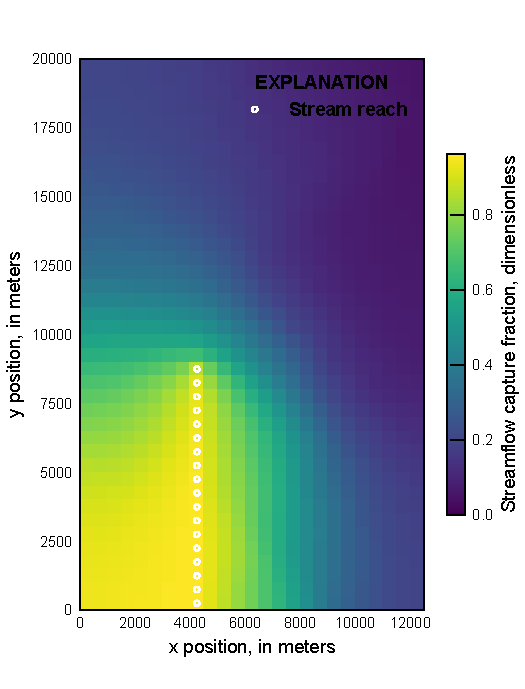
\includegraphics{Figures/sfr-capture.pdf}
	\caption{Streamflow capture fraction simulated for the synthetic valley
	model, the fraction of a withdrawal at a cell that is drawn from the stream
	rather than from storage or from another boundary, for the model layer in
	which it is largest. Open circles mark the cells the streamflow routing
	package occupies. Capture is reported for a withdrawal applied through the
	final stress period, and the reach depths are solved with the flow equations
	as described in this chapter.}
	\label{fig:sfr-capture}
\end{figure}

The synthetic valley model was pumped and the resulting change in streamflow compared with the difference between two forward runs. Capture fractions across the model are shown in figure~\ref{fig:sfr-capture}. Holding the reach depths fixed gave a discrepancy of about 26\%. Solving the reach equations with the flow equations reduced it to 0.04\%.

A branching network, in which one reach receives water from two upstream reaches and the apportionment fractions therefore matter, reproduces its finite-difference sensitivities to the same tolerance.

\section*{Limitations}

Two cases are left with a fixed depth, and \adj{} reports each rather than returning a partial derivative silently.

A reach with more than one cross-section point takes its discharge from a section rating rather than from equation~\ref{eqn:sfr-manning}, so the exponent in equation~\ref{eqn:sfr-dqdd} does not hold. The station, height, and roughness that define the section are available, so the rating can be reproduced and differentiated.

A diversion removes water from a reach under one of four rules, each with a simple derivative in the flow available to it, and each scaling a routing coefficient the reach equations already carry. Which rule is in effect is not currently recoverable from the simulation, so the derivative cannot be selected.
